% !TeX program = pdflatex
\documentclass[11pt,a4paper]{article}

% =========================================================
% PACKAGES (FAST / OVERLEAF-SAFE)
% =========================================================
\usepackage[T1]{fontenc}
\usepackage[utf8]{inputenc}
\usepackage[english]{babel}

\usepackage{geometry}
\geometry{margin=2.2cm}

\usepackage{amsmath,amssymb,mathtools,bm}
\usepackage{microtype}
\usepackage{lmodern}
\usepackage{parskip}

\usepackage{xcolor}
\usepackage{hyperref}
\usepackage{booktabs}
\usepackage{tabularx}
\usepackage{enumitem}

\usepackage{tcolorbox}
\tcbuselibrary{skins,breakable}

\usepackage{tikz}
\usetikzlibrary{arrows.meta}

% =========================================================
% COLORS / THEME
% =========================================================
\definecolor{Navy}{HTML}{061C3A}
\definecolor{Panel}{HTML}{0B2A4D}
\definecolor{Line}{HTML}{244A74}
\definecolor{Text}{HTML}{EAF2FF}
\definecolor{Muted}{HTML}{A9BBDC}

% Greek / risk factor colors
\definecolor{Delta}{RGB}{0,160,255}
\definecolor{Gamma}{RGB}{60,220,120}
\definecolor{Theta}{RGB}{255,90,90}
\definecolor{Vega}{RGB}{190,120,255}
\definecolor{Rho}{RGB}{255,200,0}
\definecolor{Credit}{RGB}{255,140,0}
\definecolor{Corr}{RGB}{0,220,200}
\definecolor{Div}{RGB}{180,180,180}

\hypersetup{
  colorlinks=true,
  linkcolor=Delta,
  urlcolor=Delta
}

% =========================================================
% BOXES (FEW, FAST)
% =========================================================
\newtcolorbox{defbox}[1][]{
  enhanced, breakable,
  colback=white,
  colframe=Line,
  boxrule=0.8pt,
  arc=2mm,
  left=3mm,right=3mm,top=2mm,bottom=2mm,
  title=\textbf{Definition},
  #1
}
\newtcolorbox{insightbox}[1][]{
  enhanced, breakable,
  colback=white,
  colframe=black!12,
  boxrule=0.7pt,
  arc=2mm,
  left=3mm,right=3mm,top=2mm,bottom=2mm,
  title=\textbf{Desk intuition},
  #1
}
\newtcolorbox{warningbox}[1][]{
  enhanced, breakable,
  colback=white,
  colframe=Theta,
  boxrule=0.9pt,
  arc=2mm,
  left=3mm,right=3mm,top=2mm,bottom=2mm,
  title=\textbf{Pitfall / risk},
  #1
}
\newtcolorbox{atlasbox}[1][]{
  enhanced, breakable,
  colback=Panel,
  colframe=Line,
  boxrule=0.8pt,
  arc=2mm,
  left=3mm,right=3mm,top=2.2mm,bottom=2.2mm,
  #1
}
\newtcolorbox{subcatbox}[2][]{
  enhanced, breakable,
  colback=white,
  colframe=#2,
  boxrule=0.9pt,
  arc=2mm,
  left=3mm,right=3mm,top=2mm,bottom=2mm,
  #1
}

% =========================================================
% TAGS (FAST)
% =========================================================
\newcommand{\Tag}[2]{%
  \begingroup
  \setlength{\fboxsep}{2.2pt}%
  \fcolorbox{#2}{#2!10}{\textcolor{#2}{\scriptsize\bfseries #1}}%
  \endgroup
}

\newcommand{\GreekSig}[5]{%
  \Tag{$\Delta$\,#1}{Delta}\;
  \Tag{$\Gamma$\,#2}{Gamma}\;
  \Tag{$\Theta$\,#3}{Theta}\;
  \Tag{$\nu$\,#4}{Vega}\;
  \Tag{$\rho$\,#5}{Rho}%
}

\newcommand{\RiskTags}[1]{#1}

\newcommand{\Primary}[1]{\Tag{Primary: #1}{#1}}

% =========================================================
% PRODUCT ENTRY (light, no per-product tcolorbox)
% =========================================================
\newcommand{\Prod}[7]{%
\textbf{#1}\hfill \Primary{#2}\\
\textbf{Typical sensitivities at initiation:}\; #3\\
\textbf{Economic structure:} #4\\
\textbf{Payoff at maturity (schematic):} #5\\
\textbf{What you are trading (Greeks / risk premia):} #6\\
\textbf{Key risks / notes:} #7\\[1.4mm]
}

% =========================================================
% LIGHT PAYOFF DRAWING HELPERS (NO PGFPLOTS)
% =========================================================
\newcommand{\PayoffAxes}[3]{% xmin xmax title
\draw[->,line width=0.7pt] (#1,0) -- (#2,0) node[below] {\small $S_T$};
\draw[->,line width=0.7pt] (0,-1.3) -- (0,2.3) node[left] {\small Payoff};
\node[anchor=west] at (#1,2.05) {\small\bfseries #3};
}
\newcommand{\Kmark}[2]{% x label
\draw[line width=0.6pt] (#1,-0.12) -- (#1,0.12);
\node[below] at (#1,-0.12) {\scriptsize #2};
}

% =========================================================
% DOCUMENT
% =========================================================
\begin{document}

% =========================================================
% COVER + DASHBOARD (dark)
% =========================================================
\begin{titlepage}
\pagecolor{Navy}\color{Text}

\vspace*{1.4cm}
{\Huge\bfseries Structured Products Atlas}\\[2mm]
{\Large\color{Muted}Classic building blocks mapped to Greeks \& risk premia}\\[6mm]

\begin{atlasbox}
\textbf{Legend (dominant driver)}\quad
\Tag{Delta}{Delta}\;
\Tag{Gamma}{Gamma}\;
\Tag{Theta}{Theta}\;
\Tag{Vega}{Vega}\;
\Tag{Rho}{Rho}\;
\Tag{Credit}{Credit}\;
\Tag{Corr}{Correlation}\;
\Tag{Div}{Dividends}
\vspace{1mm}

\color{Muted}\small
Structured notes are typically \textbf{Bond + Options} (plus issuer credit).
Beyond Greeks, desks monitor \textbf{credit spread}, \textbf{equity skew}, \textbf{dividends}, \textbf{correlation} (multi-asset), and \textbf{gap / barrier risk}.
\end{atlasbox}

\vspace{4mm}

\begin{atlasbox}
\color{Text}
\begingroup
\renewcommand{\arraystretch}{1.18}
\begin{tabularx}{\textwidth}{@{}X X X X@{}}
\toprule
\textbf{\Large Capital Protected} & \textbf{\Large Yield / Income} & \textbf{\Large Autocallables} & \textbf{\Large Exotics / Multi-asset} \\
\midrule
\textcolor{Rho}{Capital Protected Note (CPN)}\par
\textcolor{Delta}{Participation Note}\par
\textcolor{Delta}{Capped Participation / Call Spread Note}\par
\textcolor{Gamma}{Cliquet / Ratchet Note}\par
\textcolor{Delta}{CPPI (dynamic protection)}\par

&
\textcolor{Theta}{Reverse Convertible}\par
\textcolor{Theta}{Discount Certificate / Discount Note}\par
\textcolor{Theta}{Covered Call Note}\par
\textcolor{Theta}{Bonus Certificate / Bonus Cap}\par
\textcolor{Theta}{Range Accrual / Digital Coupon Note}\par
\textcolor{Vega}{Variance / Vol-linked Note (concept)}\par

&
\textcolor{Theta}{Autocall (Athena style)}\par
\textcolor{Theta}{Phoenix Note (conditional coupons)}\par
\textcolor{Theta}{Autocallable on Worst-of (multi-asset)}\par
\textcolor{Vega}{Callable / Bermudan features (concept)}\par

&
\textcolor{Corr}{Worst-of / Best-of / Basket Note}\par
\textcolor{Vega}{Barrier Note (KI / KO)}\par
\textcolor{Div}{Quanto Note (FX adjustment)}\par
\textcolor{Gamma}{Asian / Averaging Note}\par
\textcolor{Rho}{CMS Steepener (rates)}\par
\\
\bottomrule
\end{tabularx}
\endgroup
\end{atlasbox}

\vfill
{\small\color{Muted}Designed to compile fast on Overleaf free tier (light TikZ, no pgfplots).}
\end{titlepage}

\nopagecolor
\color{black}

\tableofcontents
\newpage

% =========================================================
\section{1. Structured products = bond + options (+ credit)}

\subsection{1.1 The universal decomposition}
\begin{defbox}
\textbf{Desk decomposition.}
A classic structured note payoff can often be written as:
\[
\text{Note} \;\approx\; \underbrace{\text{Zero-coupon bond}}_{\rho \text{ / rates}} \;+\;
\underbrace{\text{Portfolio of options}}_{\Delta,\Gamma,\Theta,\nu} \;+\;
\underbrace{\text{Issuer credit adjustment}}_{\text{Credit spread}}.
\]
\end{defbox}

\begin{insightbox}
\textbf{Why this matters in interviews / pricing.}
If you can decompose a note into vanillas (calls/puts/digitals/barriers), you can:
(i) understand the \emph{Greek profile}, (ii) hedge with listed options, and (iii) explain where the margin/coupon comes from (typically: selling convexity or vol).
\end{insightbox}

\subsection{1.2 Greeks and extra risk factors}
\begin{defbox}
\textbf{Greeks (core).}
\[
\Delta=\frac{\partial V}{\partial S},\quad
\Gamma=\frac{\partial^2 V}{\partial S^2},\quad
\Theta=\frac{\partial V}{\partial t},\quad
\nu=\frac{\partial V}{\partial \sigma},\quad
\rho=\frac{\partial V}{\partial r}.
\]
\end{defbox}

\begin{insightbox}
\textbf{In structured products, Greeks are not enough.}
\begin{itemize}[leftmargin=*,itemsep=1mm]
\item \Tag{Credit}{Credit spread}: note valuation depends on issuer curve (especially long maturities).
\item \Tag{Div}{Dividends}: single-name equity notes are very dividend-sensitive (forward level shifts).
\item \Tag{Corr}{Correlation}: basket / worst-of notes embed correlation and tail dependence.
\item \Tag{Vega}{Skew / smile}: barrier and autocall features are extremely skew-sensitive (downside IV).
\item Gap risk: barriers + discrete observation create jump / gap exposure beyond diffusive Greeks.
\end{itemize}
\end{insightbox}

\begin{warningbox}
\textbf{Never forget: issuer credit risk.}
A “capital protected” note protects capital \emph{only if the issuer does not default}.
\end{warningbox}

% =========================================================
\section{2. Payoff intuition (fast schematics)}

\subsection{2.1 Capital protected participation (floor + upside)}
\begin{center}
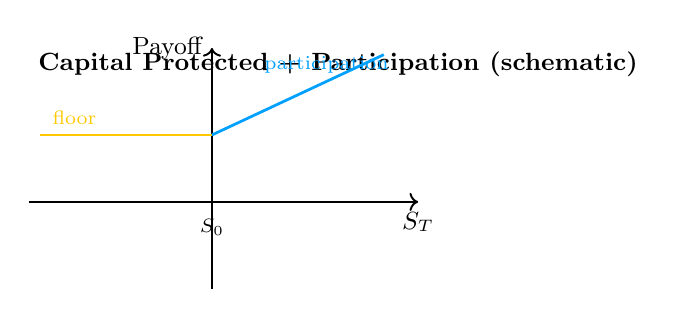
\begin{tikzpicture}[x=0.06\textwidth,y=0.85cm]
\PayoffAxes{-3.2}{3.6}{Capital Protected + Participation (schematic)}
\Kmark{0}{$S_0$}
% floor at 1, then linear
\draw[line width=1.0pt,Rho] (-3,1) -- (0,1);
\draw[line width=1.0pt,Delta] (0,1) -- (3,2.2);
\node[Rho] at (-2.4,1.25) {\scriptsize floor};
\node[Delta] at (2.0,2.05) {\scriptsize participation};
\end{tikzpicture}
\end{center}

\subsection{2.2 Reverse convertible (coupon + short put flavor)}
\begin{center}
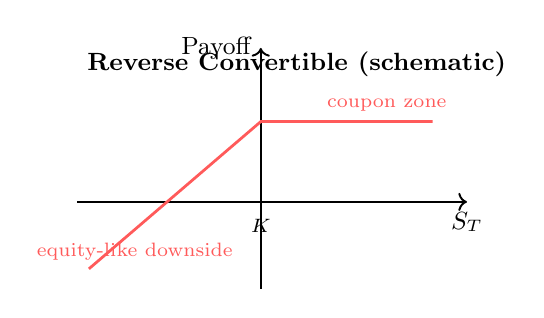
\begin{tikzpicture}[x=0.06\textwidth,y=0.85cm]
\PayoffAxes{-3.2}{3.6}{Reverse Convertible (schematic)}
\Kmark{0}{$K$}
% flat then linear down
\draw[line width=1.0pt,Theta] (-3,-1.0) -- (0,1.2) -- (3,1.2);
\node[Theta] at (2.2,1.45) {\scriptsize coupon zone};
\node[Theta] at (-2.2,-0.75) {\scriptsize equity-like downside};
\end{tikzpicture}
\end{center}

\subsection{2.3 Autocall idea (path dependent, schematic at maturity)}
\begin{center}
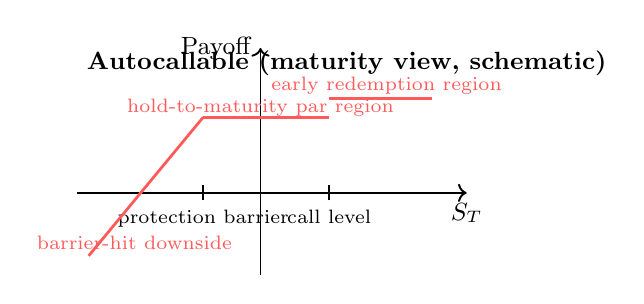
\begin{tikzpicture}[x=0.06\textwidth,y=0.8cm]
\PayoffAxes{-3.2}{3.6}{Autocallable (maturity view, schematic)}
\Kmark{1.2}{call level}
\Kmark{-1.0}{protection barrier}
% above call level: redeemed at par+coupon
\draw[line width=1.0pt,Theta] (1.2,1.5) -- (3,1.5);
% between barrier and call: par+coupon at maturity
\draw[line width=1.0pt,Theta] (-1.0,1.2) -- (1.2,1.2);
% below barrier: downside participation
\draw[line width=1.0pt,Theta] (-3,-1.0) -- (-1.0,1.2);
\node[Theta] at (2.2,1.7) {\scriptsize early redemption region};
\node[Theta] at (0,1.35) {\scriptsize hold-to-maturity par region};
\node[Theta] at (-2.2,-0.8) {\scriptsize barrier-hit downside};
\end{tikzpicture}
\end{center}

% =========================================================
\section{3. Product catalogue (classic structured notes)}

% =========================================================
\subsection{3.1 Capital protected family}

\begin{subcatbox}[title=\textbf{Capital Protected Notes (CPN) \& Participation}]{Rho}

\Prod
{Capital Protected Note (CPN) --- principal protected at maturity}
{Rho}
{\GreekSig{+}{+}{-}{+}{+}\;\; \RiskTags{\Tag{Credit}{Credit}}}
{Buy a zero-coupon bond that grows to 100\% at $T$ + use remaining budget to buy calls (or call spread).}
{Floor at 100\% (issuer-dependent) + upside participation via call(s).}
{Mainly \Tag{Rho}{Rho} (bond), plus \Tag{Vega}{Vega} and \Tag{Gamma}{Gamma} from the long call.}
{Credit risk of issuer; upside depends on implied vol level; dividends reduce forward (equity); liquidity/fees matter.}

\Prod
{Participation Note (uncapped)}
{Delta}
{\GreekSig{+}{+}{-}{+}{+}\;\; \RiskTags{\Tag{Credit}{Credit}\;\Tag{Div}{Div}}}
{Bond + long call struck near $S_0$ (or forward strike).}
{At maturity: floor (via bond) + near-linear upside above strike.}
{You are \emph{buying} \Tag{Vega}{Vega} and \Tag{Gamma}{Gamma}.}
{If IV collapses after issuance, mark-to-market can drop even if spot unchanged. Dividend forecast errors can shift forward and effective participation.}

\Prod
{Capped Participation / Call Spread Note}
{Delta}
{\GreekSig{+}{(reduced)}{-}{(reduced)}{+}\;\; \RiskTags{\Tag{Credit}{Credit}}}
{Bond + long call at $K_1$ and short call at $K_2>K_1$.}
{Upside is capped; cheaper than uncapped participation.}
{Delta exposure in a band; Vega/Gamma reduced vs uncapped because of the short call.}
{Cap is the trade-off: in strong rallies you underperform. Short call adds skew exposure and (equity) assignment considerations if physically-settled.}

\Prod
{Cliquet / Ratchet Note (equity cliquet)}
{Gamma}
{\GreekSig{(varies)}{+}{-}{+}{(small)}\;\; \RiskTags{\Tag{Vega}{Skew}\;\Tag{Credit}{Credit}}}
{Often replicable as a sum of periodically reset options with caps/floors on each period return.}
{Path-dependent: locks in periodic gains; often has local caps and a global floor.}
{Long \Tag{Gamma}{Gamma} / \Tag{Vega}{Vega} (you benefit from realized vol if structure is long optionality), but details depend on cap/floor.}
{Complexity: realized vol, monitoring dates, and smile dynamics matter. Pricing is model-dependent (local vol / stochastic vol).}

\Prod
{CPPI (Constant Proportion Portfolio Insurance)}
{Delta}
{\GreekSig{+}{(varies)}{(varies)}{(varies)}{+}\;\; \RiskTags{\Tag{Credit}{Credit}\;\Tag{Vega}{Gap risk}}}
{Dynamic allocation between risky asset and cash to maintain a floor; leverage proportional to cushion.}
{Not an option payoff: dynamic strategy aiming at capital protection.}
{Dominant driver is Delta (allocation), with strong sensitivity to jumps and rebalancing rules.}
{Gap risk can break protection; liquidity constraints, transaction costs, and rebalancing frequency are crucial.}
\end{subcatbox}

% =========================================================
\subsection{3.2 Yield enhancement / income notes}

\begin{subcatbox}[title=\textbf{Yield / Income (you are usually selling optionality)}]{Theta}

\Prod
{Reverse Convertible}
{Theta}
{\GreekSig{+}{-}{+}{-}{+}\;\; \RiskTags{\Tag{Credit}{Credit}\;\Tag{Div}{Div}\;\Tag{Vega}{Skew}}}
{Bond + short put (often ATM/OTM) \;(+ coupon funded by put sale).}
{If $S_T\ge K$: redeemed near par + coupons. If $S_T<K$: investor receives shares or suffers equity-linked loss.}
{You are selling \Tag{Vega}{Vega} and \Tag{Gamma}{Gamma} (short put), harvesting \Tag{Theta}{Theta}.}
{Downside tail risk dominates. Equity skew makes downside IV expensive: coupon largely comes from selling crash protection.}

\Prod
{Discount Certificate / Discount Note}
{Theta}
{\GreekSig{+}{-}{+}{-}{+}\;\; \RiskTags{\Tag{Credit}{Credit}\;\Tag{Div}{Div}}}
{Economically similar to: long underlying exposure + short call (cap) and/or short put depending on exact certificate.}
{Buy at a discount, upside capped.}
{Carry-oriented: you typically sell some optionality to get the discount (short Vega).}
{Cap risk (miss strong rally). Model: dividend/forward matters a lot for the discount.}

\Prod
{Covered Call Note}
{Theta}
{\GreekSig{+}{-}{+}{-}{+}\;\; \RiskTags{\Tag{Credit}{Credit}\;\Tag{Div}{Div}}}
{Bond + short call (or long asset + short call via note).}
{Upside capped; coupon enhanced.}
{You sell upside convexity (short Gamma on rallies) and short Vega; earn Theta.}
{In trending bull markets, underperforms; gap up can produce quick mark-to-market loss on short call.}

\Prod
{Bonus Certificate / Bonus Cap}
{Theta}
{\GreekSig{+}{(state-dependent)}{+}{(often -)}{+}\;\; \RiskTags{\Tag{Vega}{Barrier/Skew}\;\Tag{Credit}{Credit}}}
{Typical replication intuition: long underlying exposure + short down-and-in put (barrier) + possibly short call for cap.}
{If barrier not breached: payoff at least bonus level (and maybe capped). If breached: behaves more like underlying (or discounted).}
{Often: you earn carry by being short downside barrier optionality (short Vega near barrier, short Gamma around barrier region).}
{Discrete monitoring + gap risk make hedging hard; barrier probability depends strongly on skew and local vol model.}

\Prod
{Range Accrual / Digital Coupon Note}
{Theta}
{\GreekSig{0}{-}{+}{-}{+}\;\; \RiskTags{\Tag{Vega}{Smile}\;\Tag{Credit}{Credit}}}
{Coupon accrues when $S_t$ stays within a range (or if $S_T$ is above/below a level). Replicable with digitals / tight spreads.}
{Highly non-linear: coupon depends on time spent in region / indicator events.}
{Short Gamma around boundaries (range edges); short Vega; earns Theta in calm markets.}
{If spot hugs the boundary, hedging becomes unstable. Discrete observation makes it “jump sensitive”.}

\Prod
{Variance / Vol-linked Note (concept)}
{Vega}
{\GreekSig{0}{+}{-}{+}{(small)}\;\; \RiskTags{\Tag{Vega}{Vol of vol}\;\Tag{Credit}{Credit}}}
{Notes linked to realized variance (or implied variance) via swaps/option replication.}
{Payoff tied to realized variance level.}
{Pure vol exposure: long or short Vega depending on structure.}
{Path dependence (realized variance), jumps, and volatility-of-vol dominate.}
\end{subcatbox}

% =========================================================
\subsection{3.3 Autocallables (the classic flow product)}

\begin{subcatbox}[title=\textbf{Autocallables (Athena / Phoenix family)}]{Theta}

\Prod
{Autocall (Athena style: unconditional or simple coupons)}
{Theta}
{\GreekSig{+}{-}{+}{-}{+}\;\; \RiskTags{\Tag{Credit}{Credit}\;\Tag{Vega}{Skew}\;\Tag{Div}{Div}}}
{Bond + short option package with early redemption (knock-out) features; coupon funded by selling optionality.}
{If underlying above call level on an observation date: early redeem at par + coupon. Else continues.}
{Structurally short Vega and short Gamma: coupons are funded by selling convexity/vol + path dependence.}
{Model risk: local vol vs stochastic vol changes call probabilities; discrete observation makes hedging jumpy. Dividend curve matters.}

\Prod
{Phoenix Note (conditional coupons + protection barrier, often worst-of)}
{Theta}
{\GreekSig{(tilted)}{-}{+}{-}{+}\;\; \RiskTags{\Tag{Credit}{Credit}\;\Tag{Corr}{Correlation}\;\Tag{Vega}{Downside skew}}}
{Autocall + conditional coupons (paid if underlying above a coupon barrier) + capital protection barrier (often KI).}
{If barriers respected: coupons paid and possibly early redemption. If protection barrier breached: downside participation at maturity (often worst-of).}
{You are selling downside skew and correlation (worst-of); dominant drivers are short Vega, short Gamma, long Theta.}
{Worst-of makes correlation/tail dependence crucial. Stress in crises: correlation goes to 1, skew steepens, and gap risk hits barriers.}

\Prod
{Autocallable on Worst-of Basket}
{Corr}
{\GreekSig{(complex)}{-}{+}{-}{+}\;\; \RiskTags{\Tag{Corr}{Correlation}\;\Tag{Vega}{Skew}\;\Tag{Credit}{Credit}}}
{Same autocall logic but referencing worst performer of a basket.}
{Maturity payoff depends on worst-of; early redemption depends on basket condition (varies).}
{Short correlation is typically embedded (cheap to issuer when correlation is high in stress).}
{Hedging requires basket greeks + correlation/dispersion hedges; worst-of is tail-heavy and very skew-sensitive.}

\Prod
{Callable / Bermudan feature (concept)}
{Vega}
{\GreekSig{(varies)}{(varies)}{(varies)}{(varies)}{+}\;\; \RiskTags{\Tag{Vega}{Model risk}\;\Tag{Credit}{Credit}}}
{Issuer has call rights at multiple dates; economically a Bermudan option on the note value.}
{Payoff depends on optimal exercise policy of issuer.}
{Strong model dependence: exercise boundary + vol term structure.}
{Callable features can flip carry profile; always ask: who holds the option to call? issuer or investor.}
\end{subcatbox}

% =========================================================
\subsection{3.4 Exotics / Multi-asset / FX / Rates}

\begin{subcatbox}[title=\textbf{Exotics and cross-asset classics}]{Vega}

\Prod
{Barrier Note (KI / KO, down-and-in / down-and-out)}
{Vega}
{\GreekSig{(state)}{(state)}{(state)}{(very sensitive)}{+}\;\; \RiskTags{\Tag{Vega}{Skew}\;\Tag{Credit}{Credit}}}
{Vanilla options replaced by barrier options (discrete monitoring in practice).}
{If barrier hit/not hit: payoff switches regime (knock-in/out).}
{Barriers are extremely skew- and local-vol-sensitive; hedging near barrier is hard (Gamma spikes).}
{Gap risk: a jump can cross barrier without trading through it. Observation schedule matters.}

\Prod
{Worst-of / Best-of / Basket Note}
{Corr}
{\GreekSig{(complex)}{(complex)}{(often +)}{(complex)}{+}\;\; \RiskTags{\Tag{Corr}{Correlation}\;\Tag{Vega}{Skew}\;\Tag{Credit}{Credit}}}
{Payoff depends on min/max or weighted basket; common in retail structured products.}
{Worst-of concentrates downside on weakest asset; best-of concentrates upside.}
{Correlation and tail dependence dominate.}
{Dispersion/correlation hedges are needed; crises change correlation regime abruptly.}

\Prod
{Quanto Note (FX-adjusted payoff)}
{Div}
{\GreekSig{+}{+}{(varies)}{+}{+}\;\; \RiskTags{\Tag{Div}{FX quanto adj.}\;\Tag{Credit}{Credit}}}
{Payoff linked to foreign underlying but settled in domestic currency at fixed FX (quanto).}
{Investor gets foreign performance without FX exposure (apparently).}
{Actually embeds an adjustment depending on FX vol and correlation between underlying and FX.}
{Key risks: FX vol, equity--FX correlation, and dividend/forward consistency.}

\Prod
{Asian / Averaging Note}
{Gamma}
{\GreekSig{(smoother)}{(reduced)}{(varies)}{(reduced)}{+}\;\; \RiskTags{\Tag{Vega}{Model}\;\Tag{Credit}{Credit}}}
{Options written on an average price (arithmetic/geometric).}
{Payoff depends on average level, smoother than vanilla.}
{Averaging reduces Gamma/Vega vs vanilla, but introduces path dependence.}
{Pricing/hedging can use approximations; monitoring schedule matters.}

\Prod
{CMS Steepener (rates structured note)}
{Rho}
{\GreekSig{0}{0}{(carry)}{(depends)}{+}\;\; \RiskTags{\Tag{Rho}{Rates}\;\Tag{Credit}{Credit}}}
{Coupon linked to CMS spread / curve slope (e.g., $a \times (CMS_{10}-CMS_2)$ with caps/floors).}
{Payoff depends on interest-rate curve evolution (and convexity adjustments).}
{Dominant sensitivities: rates level, curve, convexity (model).}
{Often includes callable/KO features; rate vol and correlation across tenors matter.}
\end{subcatbox}

% =========================================================
\section{4. Master checklist (what drives the coupon?)}

\begin{insightbox}
\textbf{Rule of thumb.} In classic retail structured products, the coupon is typically funded by:
\begin{itemize}[leftmargin=*,itemsep=1mm]
\item selling \Tag{Vega}{Vega} (especially downside skew),
\item selling \Tag{Gamma}{Gamma} (convexity, barrier proximity, range boundaries),
\item embedding \Tag{Credit}{issuer credit} and fees,
\item and in baskets: selling \Tag{Corr}{correlation / tail dependence}.
\end{itemize}
If a note looks “too good”, ask: \emph{which risk is being sold?} and \emph{what happens in a gap?}
\end{insightbox}

\begin{warningbox}
\textbf{Interview-grade risk sentence (use it).}
``An autocallable / phoenix is typically long carry but structurally short convexity and short downside skew; its valuation is highly sensitive to the volatility surface, discrete barrier monitoring, correlation (worst-of), dividends, and issuer credit spread.''
\end{warningbox}

% =========================================================
\section{Appendix A. Quick mapping table (dominant driver)}

\begingroup
\small
\renewcommand{\arraystretch}{1.15}
\begin{tabularx}{\textwidth}{@{}l l l@{}}
\toprule
\textbf{Product} & \textbf{Dominant driver} & \textbf{Typical ``sold'' risk to fund coupon} \\
\midrule
Capital Protected Note & \Tag{Rho}{Rho} & none (coupon low), but \Tag{Credit}{credit} matters \\
Participation Note & \Tag{Delta}{Delta} / \Tag{Vega}{Vega} & long optionality (investor pays via reduced participation) \\
Call Spread Note & \Tag{Delta}{Delta} & upside cap (sell call) \\
Reverse Convertible & \Tag{Theta}{Theta} & short put: \Tag{Gamma}{Gamma} + \Tag{Vega}{Vega} (downside skew) \\
Discount / Covered Call Note & \Tag{Theta}{Theta} & short call (capped upside) \\
Bonus Certificate & \Tag{Theta}{Theta} & short barrier downside optionality (gap/skew) \\
Range Accrual / Digital & \Tag{Theta}{Theta} & short gamma around boundaries + short vega \\
Autocall (Athena) & \Tag{Theta}{Theta} & short vega/gamma + path dependence \\
Phoenix (worst-of) & \Tag{Theta}{Theta} + \Tag{Corr}{Corr} & short downside skew + short correlation \\
Barrier note & \Tag{Vega}{Vega} & skew + gap / monitoring risk \\
Worst-of basket & \Tag{Corr}{Corr} & tail dependence / correlation regime \\
Quanto & \Tag{Div}{FX corr} & FX vol + equity--FX correlation \\
CMS Steepener & \Tag{Rho}{Rho} & curve convexity / rate vol \\
\bottomrule
\end{tabularx}
\endgroup

\vspace{3mm}
{\footnotesize\textit{Educational material only (not investment advice).}}

\end{document}
